\section{P, NP, NP-Complete, EXP}

\label{sec:hard}
\begin{Def}[Decision Problem]

    A \textbf{decision problem} is a problem that can be answered with a simple ``yes'' or ``no'' answer.
\end{Def}

\begin{Def}[Complexity Classes]

    A \textbf{complexity class} is a set of problems of related complexity,
    solvable under the same system constraints. A problem $x$ is in complexity class $X$ if they
    share similar characteristics in complexity. A problem is \textbf{solvable} if it runs 
    in polynomial time. Notable classes:

    \begin{itemize}
        \item \textbf{P} - Solvable in polynomial time
        \item \textbf{NP} - Verifiable (``yes'') in Polynomial time (nondeterministic polynomial time).
        \item \textbf{NP-Hard} - Not necessarily NP, a decision problem, nor has a solution. 
        If a problem $H$ is NP-Hard, all problems $L$ in NP can be reduced to $H$. I.e., $H$ can run as a sub-routine solving all NP.
        It is said that NP-Hard problems are at least as hard as NP problems.
        \item \textbf{NP-Complete} - NP and NP-Hard. 
        \item \textbf{EXP} - Solvable in exponential time.
    \end{itemize}

\end{Def}

\begin{Tip}
    \textbf{Alan Turing} (1912-1954) was a British mathematician and logician. In 1936, he introduced the concept of the Turing machine, laying the groundwork for theory of computation. During World War II Turing broke the German Enigma encrypted code shifting the tides of the war. He after worked on early computers and artificial intelligence, proposing the ``Turing Test'', defining machine intelligence. Tragically, Turing's life was cut short by personal and professional persecution against his homosexuality, dying at 41.
\end{Tip}

\newpage

\begin{Example}[P, NP, NP-Hard, NP-Complete, EXP]

    \begin{itemize}
        \item \textbf{P} - Sorting algorithms.
        \item \textbf{NP} - Travelling Salesman Problem (\ref{TSP}).
        \item \textbf{NP-Hard} - Halting Problem (\ref{HaltingProblem}).
        \item \textbf{NP-Complete} - Boolean Satisfiability Problem (\ref{3-SAT}).
        \item \textbf{EXP} - Towers of Hanoi (\ref{TowersOfHanoi}), or unoptimized Fibonacci.
    \end{itemize}
\end{Example}

\begin{Func}[Halting Problem - \textit{HaltingProblem()}]

    \label{HaltingProblem}
    \vspace{-.5em}
    \begin{algorithm}[H]
        \SetAlgoLined
        \SetKwProg{Fn}{Function}{:}{\KwRet{}}
        \Fn{\textit{Halts}(program, input)}{
            \If{program(input) \textbf{doesn't halts}}{
                \Return{\text{``This program does not halt."}}
            }
            \Else{
                \While{true}{
                    \tcp{Loop forever} 
                }
            }
        }
        \KwRet{Halts(Halts, Halts)} \tcp{Run Halts on Halts with an input of itself}
    \end{algorithm}
    \noindent
    \rule{\textwidth}{0.4pt}
    \textbf{Explanation:} The Halting Problem is a decision problem that determines whether a given program will halt (terminate) or run forever on a given input. 
    This problem is undecidable, meaning there is no general algorithm that can solve the Halting Problem for all possible program-input pairs. 

    The above is an example of a paradoxical function. Line 2 checks if the program does not halt, if so, it returns that the program does not halt.
    Otherwise, it loops forever. Though if line 2 is true, that means the inner program looped forever---a contradiction---if the inner program never halted, the outer function could have never evaluated it.
    If it did halt, the outer function would have ran forever. A similar paradox, ``(1) The following statement is true. (2) The previous statement is false.''

    Despite the contrived example, the root is that given on any input it is impossible to automatically detect all cases. IDEs (Integrated Development Environments) today can detect some cases, but not all.
    Another example in the same class would be program which identifies \textbf{Dead-code} (code that won't run). These problems are NP-complete, as if dead-code is solved, then the Halting Problem could be reduced 
    to it.
\end{Func}

\begin{Tip}
    John von Neumann (1903-1957) was a Hungarian-American mathematician and polymath who made fundamental contributing to, mathematics, physics, economics, and computer science. He is best known for developing the ``\textit{Von Neumann Architecture.}''
\end{Tip}

\newpage 

\begin{Func}[3-SAT]
    
        \label{3-SAT}
        \vspace{-.5em}
        \begin{algorithm}[H]
            \SetAlgoLined
            \SetKwProg{Fn}{Function}{:}{\KwRet{}}
            \Fn{\textit{3-SAT}(formula)}{
                \For{each clause in formula}{
                    \If{clause is not satisfied}{
                        \Return{false}
                    }
                }
                \Return{true}
            }
        \end{algorithm}
        \noindent
        \rule{\textwidth}{0.4pt}
        \textbf{Explanation:} 3-SAT is a Boolean Satisfiability Problem (SAT) where each clause has exactly 3 literals. E.g.,
        $$ (x_1 \lor x_2 \lor x_3) \land (\neg x_1 \lor x_2 \lor x_3) \land \dots \land (\neg x_1 \lor \neg x_2 \lor x_3).$$

        \noindent
        $\land:=\text{AND}, \lor:=\text{OR}, \neg:=\text{NOT}$. Given an input formula, the function determines if there's a possible 
        true/false assignments to evaluate the formula to true. The best approach today is by brute-force, trying all possible assignments.

        This problem is NP-Complete, as any function could theoretically be reduced to a true-false table for which an SAT function could be solved.
        
\end{Func}

\begin{Func}[Towers of Hanoi]

    \label{TowersOfHanoi}
    \vspace{-.5em}
    \begin{algorithm}[H]
        \SetAlgoLined
        \SetKwProg{Fn}{Function}{:}{\KwRet{}}
        \Fn{\textit{TowersOfHanoi}(n, source, target, auxiliary)}{
            \If{n = 1}{
                \tcp{Move disk 1 from source to target}
            }
            \Else{
                \textit{TowersOfHanoi}(n-1, source, auxiliary, target)\;
                \tcp{Move disk n from source to target}
                \textit{TowersOfHanoi}(n-1, auxiliary, target, source)\;
            }
        }
    \end{algorithm}
    \noindent
    \rule{\textwidth}{0.4pt}
    \textbf{Explanation:} There are $n$ different sized disks stacked in decreasing order of size, and three rods. Rules:
    \textbf{(1).} One disk is moved at a time. \textbf{(2).} Each turn, a top disk moves from one stack to another. \textbf{(3).} Bigger over smaller disks are prohibited.
    Given the above, $O(2^n)$ (\ref{theo:master}).
    \begin{center}
        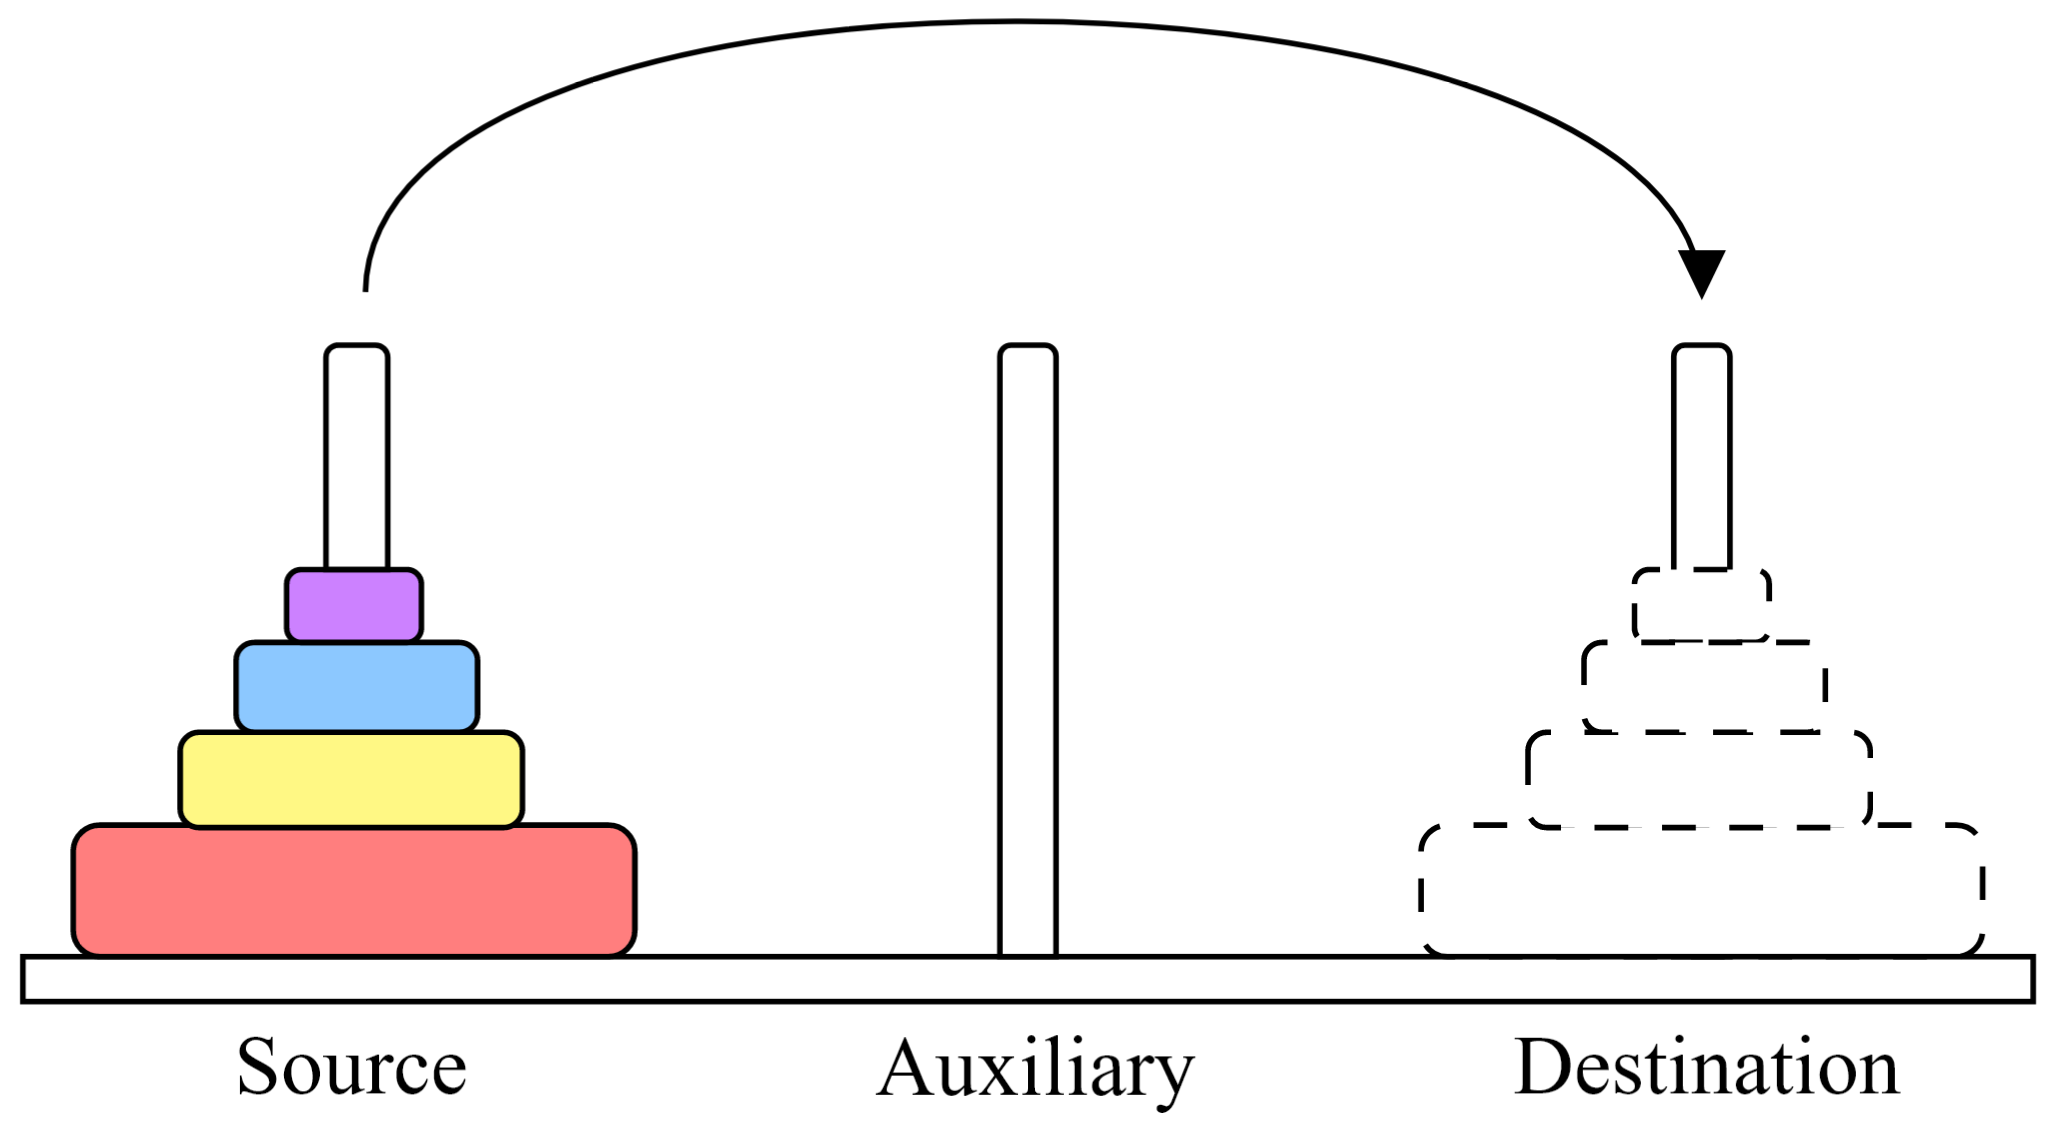
\includegraphics[width=0.55\textwidth]{Sections/hard/hanoi.png}
    \end{center}
    
\end{Func}

\newpage 

\noindent
For emphasis and clarity:
\begin{theo}[Complexity Classes Corollary]

    \begin{itemize}
        \item \textbf{P=NP, NP$\neq$P} - all P are NP as they are verifiable in polynomial time. Though as of today, no proof exists that all verifiable problems are solvable in polynomial time.
        \item \textbf{X reducing to Y} - If $X$ is solvable in $O(n^2)$ and $X$ reduces to $Y$, then $Y$ is solvable in polynomial time. However, 
        this does not grantee that $Y$ is $O(n^2)$. As $X$ is a sub-routine while $Y$'s outer function could run any number of times. For $Y$ to have $O(n^2)$ implies 
        $Y$'s main routine runs in $O(1)$.
        \item \textbf{Verification} - To verify an example is given and a criteria checked. E.g., is this path at least 10 units long?
        However to verify ``No'' requires the program to provide proof that the solution is not possible. I.e., to verify a ``No'' answer, we must check all possible solutions for which 
        we don't even know how to compute.
    \end{itemize}
\end{theo}

\begin{figure}[h!]
    \centering
    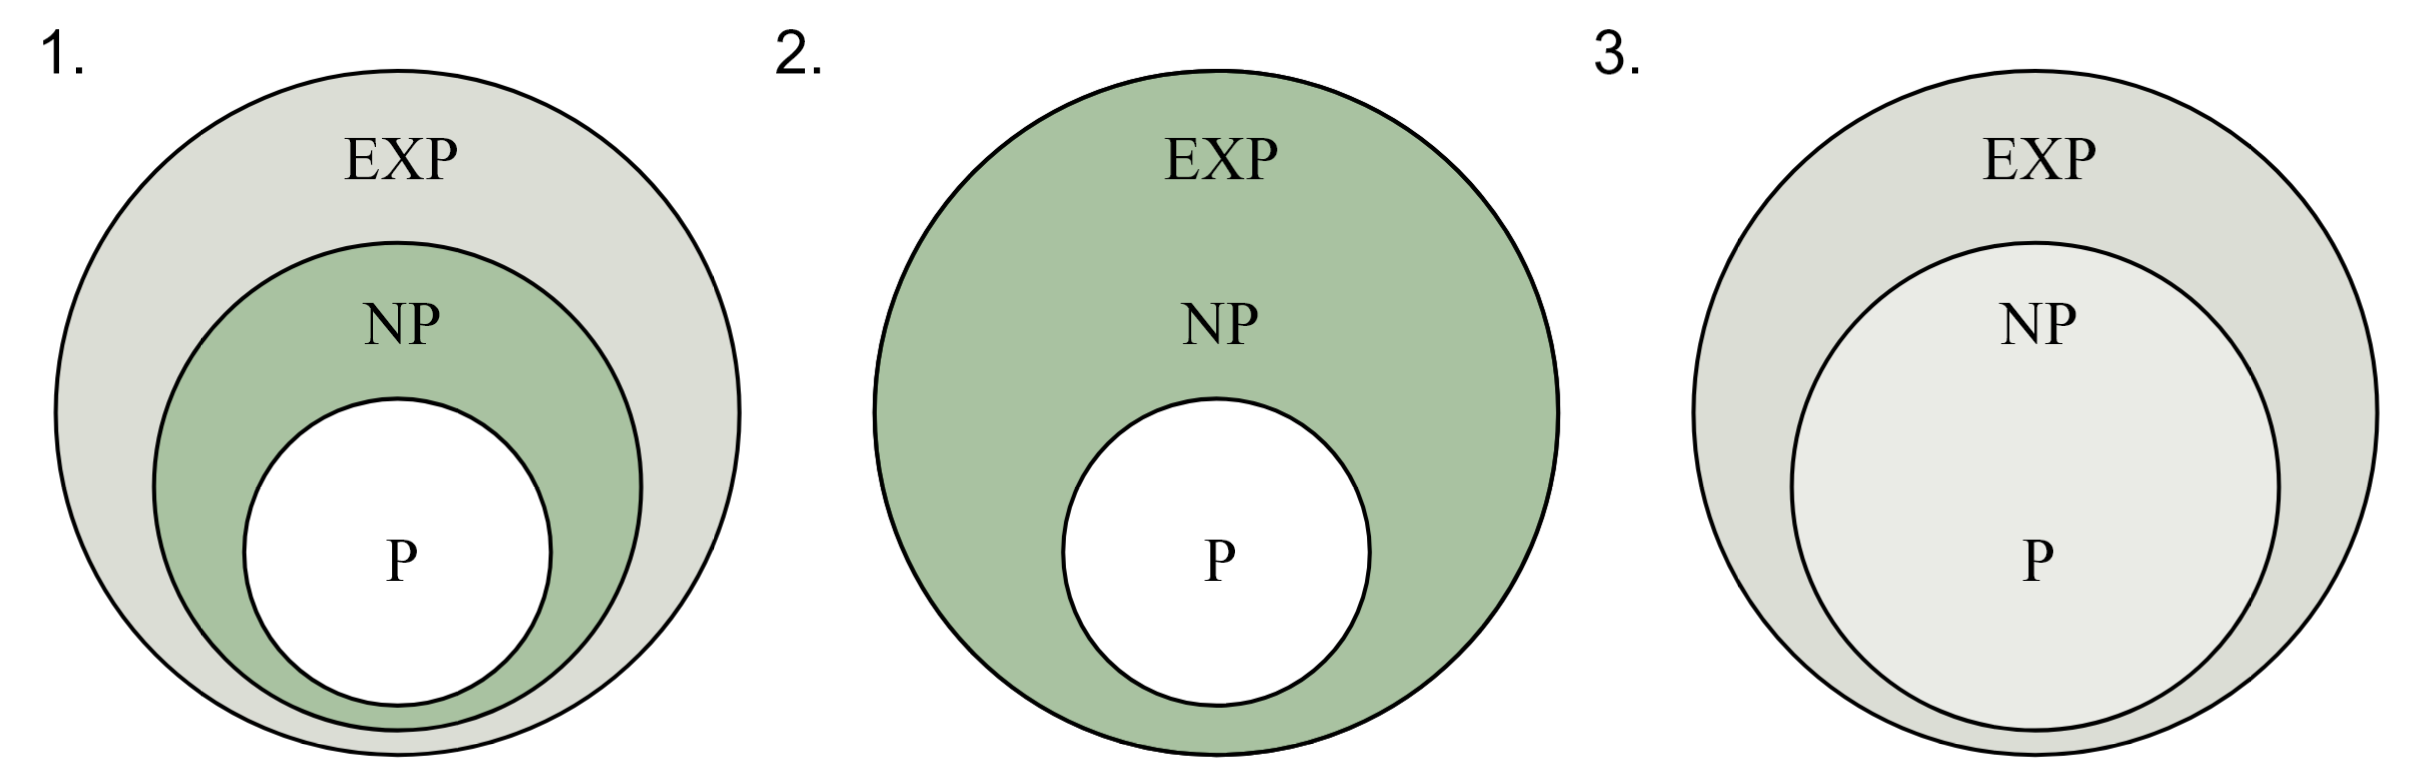
\includegraphics[width=1\textwidth]{Sections/hard/diagrams.png}
    \caption{Complexity Classes Ven Diagram of P, NP, EXP}
    \label{fig:ven}
\end{figure}

In Figure (\ref{fig:ven}), \textbf{(1)} is the general consensus on the state of complexity classes. We don't know whether 
all NP are P, or whether all EXP are NP. \textbf{(2)} shows that it could be that all EXP are NP, but we don't know. Likewise, \textbf{(3)} shows that it could be that all NP are P, but we don't know.

\newpage 
\begin{theo}[The Traveling Salesman Problem (TSP)]

    \label{TSP}

    Given a list of cities and the distances between each pair of cities, 
    what is the shortest possible route that visits each city exactly once and returns to the origin city?
    This problem is NP-Complete. 

    \begin{center}
    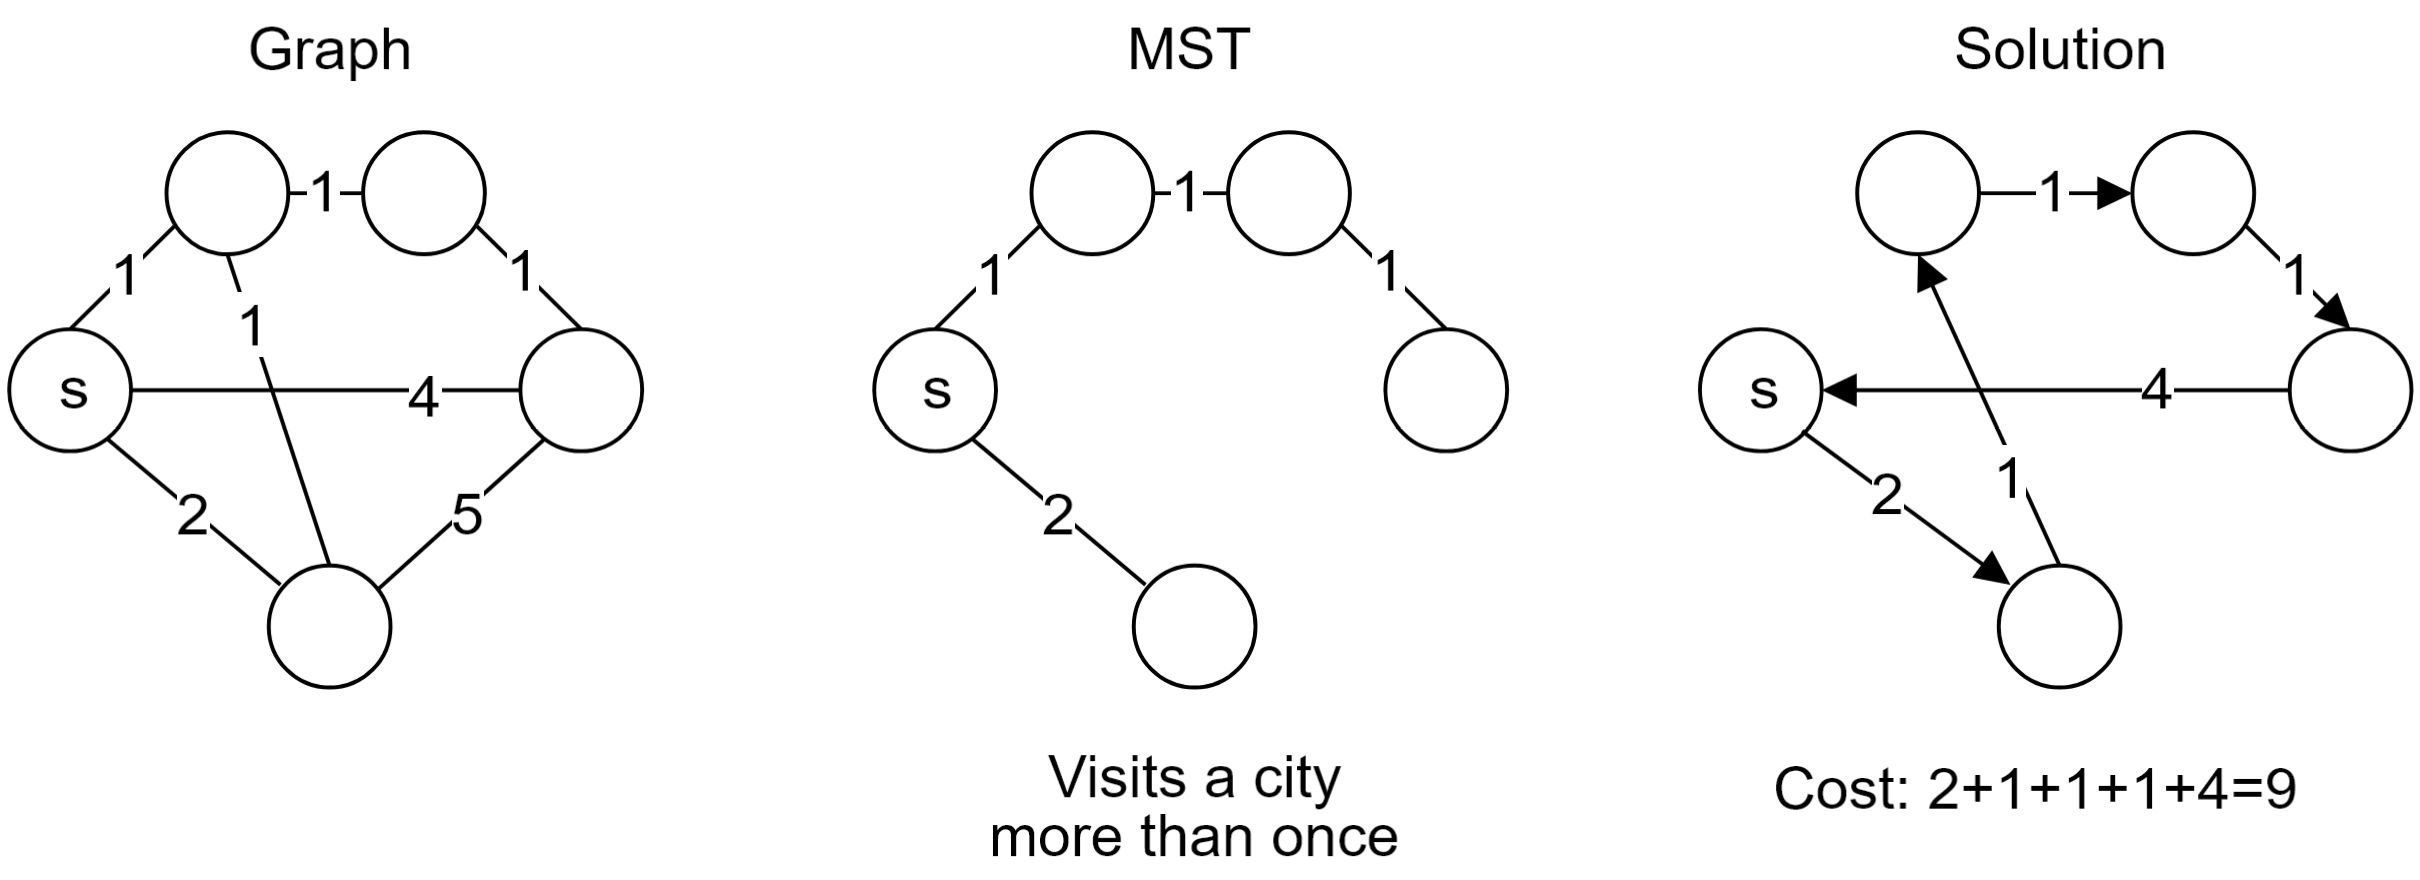
\includegraphics[width=1\textwidth]{Sections/hard/graphs.png}
    \end{center}
    \noindent
    \textbf{Note:} that this does not mean MST, as MST finds the minimal cost to connect all nodes. It isn't strictly shortest paths
    from the origin to all nodes and back, as we'd double count nodes.\\

    \noindent
    \textbf{NP Verification:}\\
    ``Does this path visit all nodes once returning to the origin in less than $k$ units?''

\end{theo}
    